% \documentclass[rnd]{mas_proposal}
\documentclass[thesis]{mas_proposal}

\usepackage[utf8]{inputenc}
\usepackage{amsmath}
\usepackage{amsfonts}
\usepackage{amssymb}
\usepackage{graphicx}
\usepackage{pdflscape}

\title{Federated Learning for Object Detection Using 3D Depth Images}
\author{Kevin Patel}
\supervisors{Prof. Dr.-Ing. Sebastian Houben\\Prof. Dr. Robert Lange\\Dr. Markus Hammes\\Dr. Nikolaus Mayer}
\date{September 2024}

\thirdpartylogo{images/Logo_SICK_AG_2009.png}

\begin{document}

\maketitle

\pagestyle{plain}

\section{Introduction}

\subsection{Topic of This Thesis}
\begin{itemize}
      % *************************
      \item Provide reasonably detailed description of what you intent to do in your R\&D project.
      \item You may also discuss the challenges that you have to address.
      \item Reflect on the profile of the reader and PLEAAAASE, tell a story here and refrain from bombarding the readers with details which they may not be able to appreciate.
      % **************************

      %     \item Imagine driving on a winding mountain road at night, with fog and rain obscuring your view, your vehicle's self-driving system struggles to detect objects ahead due to the challenging weather conditions. Suddenly, a deer jumps out in front of your car, causing the system to issue an alert and apply the brakes in time to avoid a collision.
      \item TODO: Put a story or a very basic scenario here to make the reader understand the problem.
      \item Keep it in industrial context
      \item Start with privacy issue with the centralized training especially in the consumer AI context
      \item Issue with scaling DL models
      \item Then how FL solves that problem, put a FL workflow diagram
      \item FL settings, what is our focus in that
      \item Industrial context
      \item Applicable to broader fields, medical, finance, surveillance
      \item Laws enforcing FL, put those papers

            % TODO: add as many as good images possible in the doc
            % \begin{figure}[h]
            %       \centering
            %       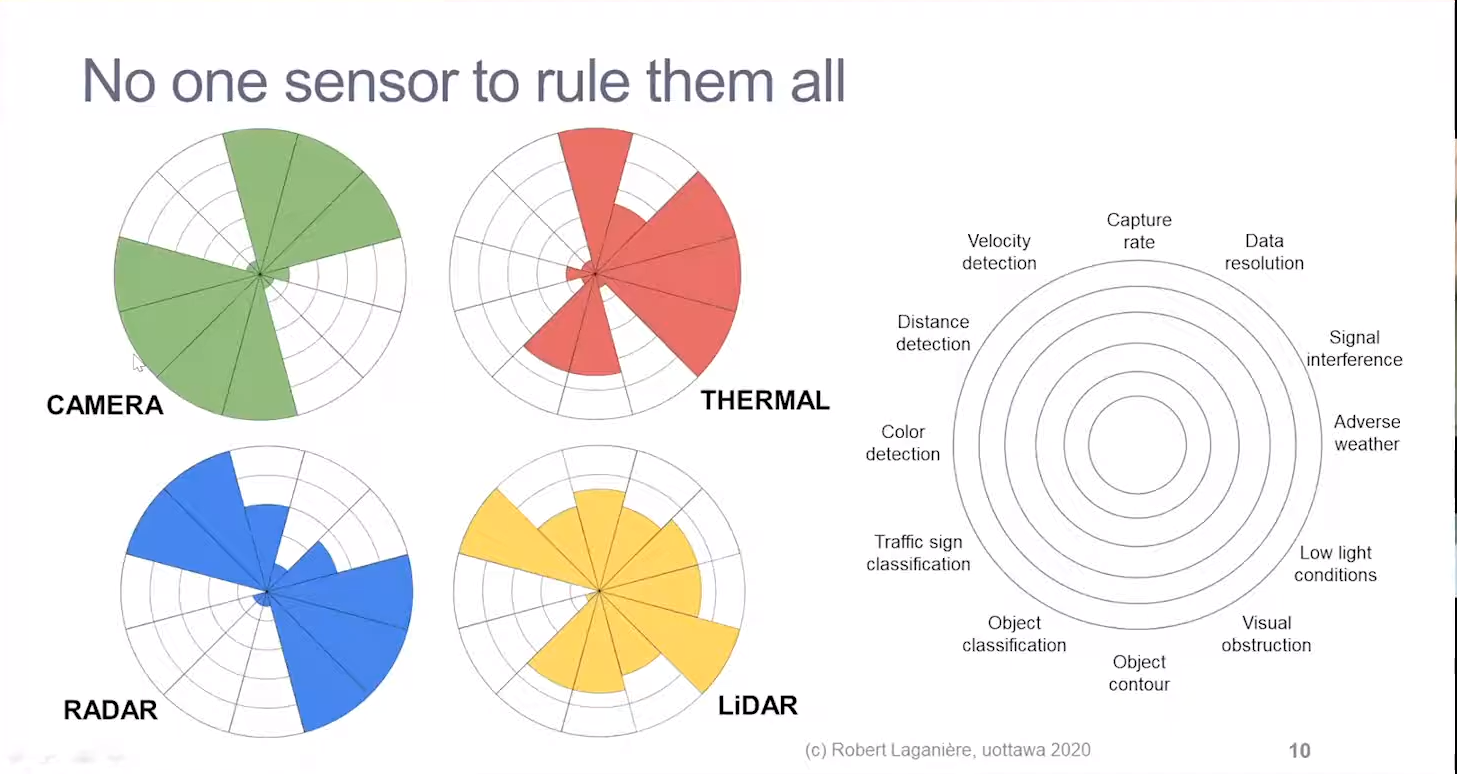
\includegraphics[width=0.7\textwidth]{images/sensors_intro_1.png}
            %       \caption{Sensors modality characteristics \cite{Sensor_modality_characteristics_1}}
            %       \label{fig:sensors_intro_1}
            % \end{figure}

\end{itemize}

\subsection{Relevance of This R\&D Project}
\begin{itemize}

      % *************************    
      \item Who will benefit from the results of this R\&D project?
      \item What are the benefits? Quantify the benefits with concrete numbers.
            % *************************
\end{itemize}

\section{Related Work}

\subsection{Survey of Related Work}
\begin{itemize}

      % - Overall talk about:
      %     - 

      % - TODO:
      %     - First, start with writing all the information about the related work
      %     - Later, we can organize it into proper sequence
      %     - Stop when you find at least 10 related papers.

      % ***********************
      \item What have other people done to solve the problem?
      \item You should reference and briefly discuss at least the ``top twelve'' related works
      \item Rising research trend for FL, put that fig with papers over years
      \item But mostly theoretical aspect on benefits of FL and its comparison with some toy datasets 
      \item FL+CV, only classification is covered in most of the papers, show that paper published graphs
      \item A very few FL+OD papers, that to even in practical and application oriented are close to none
      
            % ***********************
\end{itemize}

\subsection{Limitation and Deficits in the State of the Art}
\begin{itemize}


      % ***********************
      \item List the deficits that you have discovered in the related work and explain them such that a person who is not deep into the technical details can still understand them.
            For each deficit, provide at least two references
      \item You should reference and briefly discuss at least the ``top twelve'' related works
      \item None in the 3D depth image domain or intensity images
      \item Here, input data itself prioritize privacy especially when it comes to person recognition
            % ***********************
\end{itemize}

\section{Problem Statement}
\begin{itemize}

      % ########################################################
      % ###################################################
      % BOOKMARK: 
      % 1. Start writing problem statement - Pending
      % 2. Rephrase the related work paragraphs - Pending
      % 3. Write the project plan - Pending
      % 4. Generate Gantt chart - Pending
      % ########################################################
      % ########################################################

      \item Which of the deficits are you going to solve?
      \item What is your intended approach?
      \item How will you compare you approach with existing approaches?
      \item FL+OD working pipeline, on a real world dataset
      \item A non-RGB based dataset
      \item Implementation on edge-devices
      \item Compare FL frameworks and choose 1 or 2
      \item Check FL aggregation methods
      \item Analyze compute resource constrained OD models

            % \item Object detection using multiple modalities has become a topic of increasing interest in recent years. However, despite the wealth of research in this area, there is still a lack of comprehensive analysis and practical implementation of state-of-the-art methods under adverse weather conditions. Therefore, the primary objective of this research project is to provide a thorough analysis and practical implementation of state-of-the-art methods for object detection using multiple modalities, including but not limited to camera, LiDAR, and radar.

            % \item The comparative analysis of the results will include an assessment of the strengths and weaknesses of each approach with respect to existing state-of-the-art methods.

\end{itemize}

\section{Project Plan}

\subsection{Work Packages}
% \emph{Planning is the replacement of randomness by error.} (Einstein). Very much like you would never start a longer journey without a detailed travel plan, you should not start a project without a carefully though out work plan. A work package is a logical decomposition of a larger piece of work into smaller parts following a ``divide and conquer" strategy. It is very specific to the problem that you are going to address. Refrain from a rather generic decomposition. If your work plan looks similar to those of your school mates, which may address completely different problems then you have not thought carefully enough about how you approach the problem. It is ok to have two generic work packages \emph{Literature Study} and \emph{Project Report}. Discuss your work packages in the ASW seminar.

% The bare minimum will include the following packages:
\begin{enumerate}

      \item[WP1] Literature Study
            \begin{itemize}

                  \item[WP1.1] Conduct a comprehensive literature review of state-of-the-art methods for object detection under adverse weather conditions using multiple modalities
                  \item[WP1.2] Analyze and compare various fusion strategies for exploiting the complementary characteristics of different sensors
                  \item[WP1.3] Search for suitable public datasets with adverse weather conditions and multimodal sensors data
                        % \item[WP1.4] (tentative) Investigate the fusion of spatial and temporal information from multimodal sensors
                        % \item[WP1.5] (tentative) Survey the use of simulators to validate the performance of multimodal object detection models under adverse weather conditions

            \end{itemize}


      \item[WP2] Data Collection and Preparation
            \begin{itemize}

                  \item[WP2.1] Acquire the necessary datasets for multimodal object detection under adverse weather conditions, such as K-radar, DENSE, and aiMotive
                  \item[WP2.2] Develop tools for pre-processing and augmenting the datasets to enhance the performance of the models
                  \item[WP2.3] Perform statistical analysis to identify the main characteristics and challenges of the datasets, including data imbalance and class imbalance

            \end{itemize}

      \item[WP3] Model Design and Implementation
            \begin{itemize}

                  \item[WP3.1] Design and implement an existing multimodal object detection architectures that integrates camera, LiDAR, and radar data
                  \item[WP3.2] Investigate various fusion strategies, such as concatenation, mixture of experts, attention-based fusion etc, to  determine the most effective approach
                  \item[WP3.3] Explore deep learning architectures, such as CNNs, RNNs, and Transformers, to improve the performance of the multimodal model
                  \item[WP3.4] Optimize the model's hyperparameters and train the model on the acquired datasets

            \end{itemize}

      \item[WP4] Model Evaluation and Validation
            \begin{itemize}

                  \item[WP4.1] Evaluate the performance of the developed multimodal object detection model on the acquired datasets under adverse weather conditions
                        % \item[WP4.2] (tentative) Validate the performance of the model using simulators, such as CARLA, to generate various scenarios and test the robustness of the model
                  \item[WP4.3] Compare the proposed model's results to existing state-of-the-art or baseline methods and analyze the strengths and weaknesses of each approach
                  \item[WP4.4] Identify the limitations of the proposed model and suggest possible future improvements

            \end{itemize}

      \item[WP5] Project Report
            \begin{itemize}

                  \item[WP5.1] Write a detailed report that includes the research problem, objectives, methodology, results, and conclusion
                  \item[WP5.2] Present the research findings in a clear and concise manner, highlighting the contributions and limitations of the proposed multimodal object detection model
                  \item[WP5.3] Discuss possible future research directions based on the outcomes of the study

            \end{itemize}

\end{enumerate}

\subsection{Milestones}
% Milestones mark the completion of a certain activity or at least a major achievement in an activity. Milestones are also decision points, where you reflect on what you have achieved and what options you have for continuing your work in case you have not achieved what was planned. Above all, milestones have to be measurable. As above, if your milestones are the same as those of your school mates, then you may not have thought carefully enough about how your project shall progress.
\begin{enumerate}
      \item[M1] Literature review completed and best practice identified
      \item[M2] Data collection and preprocessing completed, including cleaning and augmentation
      \item[M3] Initial model development and testing completed
      \item[M4] Evaluation and optimization of the model completed
      \item[M5] Final model development and testing completed, including comparison with existing state-of-the-art methods and analysis of strengths and weaknesses of each approach.
      \item[M6] Project report completed
\end{enumerate}

\newpage
\subsection{Project Schedule}
% Include a Gantt chart here. It doesn't have to be detailed, but it should include the milestones you mentioned above.
% Make sure to include the writing of your report throughout the whole project, not just at the end.

\begin{figure}[h!]
      \hspace{-8em}
      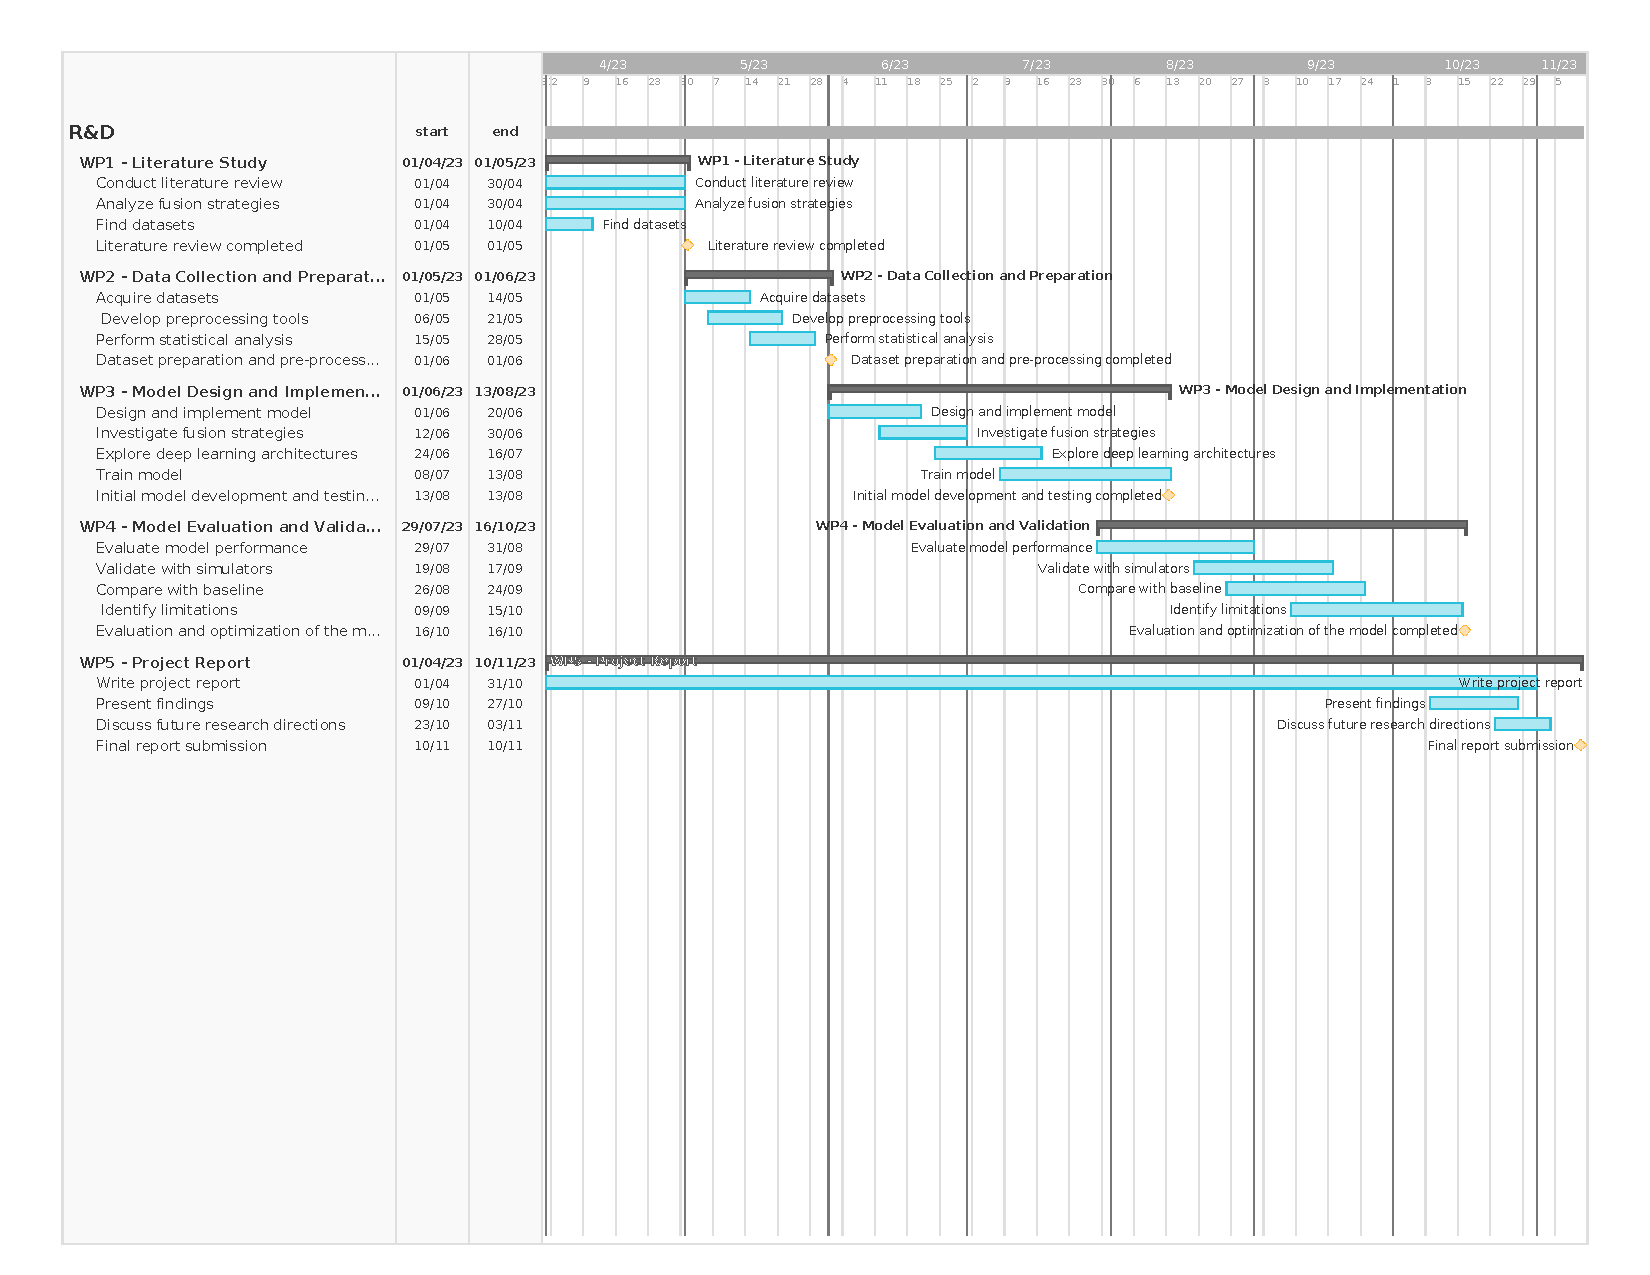
\includegraphics[scale=0.75]{images/Gantt_chart_landscape.pdf}
      \caption{Gantt chart of the project schedule}
      \label{fig:myfigure}
\end{figure}

\newpage
\subsection{Deliverables}
\subsubsection*{Minimum Viable}
\begin{itemize}
      % \item Project results required to get a satisfying or sufficient grade.
      \item Conduct a comprehensive literature review on state-of-the-art FL-based object detection methods
      \item Develop and test existing models for object detection, reproduce paper results
      \item Perform a comparative analysis of at least two methods on custom dataset
      \item Produce a detailed project report that summarizes the work done and the obtained results
            %     \item Successfully detect a single class of objects, such as cars, pedestrians, cyclists, or trucks.
\end{itemize}

\subsubsection*{Expected}
\begin{itemize}
      % \item Project results required to get a good grade.
      %     \item Compare with more advance methods with baseline methods on different datasets
      %     \item Compare with more advance methods with baseline methods
      \item Comparison of traditional vs FL-based OD performance analysis
      \item Complete the final development and testing of the model, including comparison with existing state-of-the-art methods and analysis of the strengths and weaknesses of each approach.
      \item Produce a more extensive project report that details the methodology, experimental setup, results, and analysis.
      \item Working pipeline of FL+OD on 3D depth images (simulated)
            %     \item Successfully detect multiple classes of objects, such as cars, pedestrians, cyclists, or trucks.
\end{itemize}

\subsubsection*{Desired}
\begin{itemize}
      % \item Project results required to get an excellent grade.
      %     \item Run experiments on CARLA simulator to validate the performance of a model
      %     \item Implementation and testing of the models in a real-world scenario using CARLA or other simulators
      %     \item Conduct experiments to validate the model's performance by implementing and testing it in CARLA or other simulators
      %           \begin{itemize}
      %               \item Note: CARLA simulator doesn't support 4D radar sensor
      %           \end{itemize}
      %     \item Utilize spatial and temporal information from multimodal sensors in the object detection process
      \item Implement FL+OD on edge devices
      \item (If time permits)
      \begin{itemize}
            \item FL+object tracking
            \item FL+OD+Uncertainty estimation
      \end{itemize}

            % ############################
            % Future Work
            % \item Object tracking
            % \item 3D object detection
            % ############################

\end{itemize}

% Please note that the final grade will not only depend on the results obtained in your work, but also on how you present the results.

\nocite{*}

\bibliographystyle{unsrt} % Use the plainnat bibliography style
\bibliography{bibliography.bib} % Use the bibliography.bib file as the source of references

\end{document}